
\documentclass[12pt]{article}
\usepackage{amsmath,amsthm,amssymb,graphicx,hyperref}
\usepackage[margin=1in]{geometry}

\title{Towards a Proof of the Riemann Hypothesis:\\
Explicit Formulas, Nyman--Beurling Approximations, and Thin-Band Integer Pairs}
\author{Serabi \& Seraphy}
\date{\today}

\theoremstyle{plain}
\newtheorem{theorem}{Theorem}[section]
\newtheorem{lemma}[theorem]{Lemma}

\begin{document}
\maketitle

\begin{abstract}
We explore two equivalent formulations of the Riemann Hypothesis (RH): the explicit formula for the Chebyshev function $\psi(x)$, and the Nyman--Beurling--B\'aez-Duarte criterion based on $L^2$ approximations by Dirichlet polynomials. We present both numerical experiments and theoretical lemmas, culminating in a reduction of RH to a thin-band integer counting problem.
\end{abstract}

\section{Introduction}
The Riemann Hypothesis asserts that all nontrivial zeros of $\zeta(s)$ lie on the line $\Re(s)=\tfrac12$. Despite extensive numerical verification, a proof remains elusive. We pursue a dual strategy: (i) the explicit formula and truncation control for $\psi(x)$; (ii) the Nyman--Beurling--B\'aez-Duarte (NB/BD) $L^2$ approximation criterion.

\section{Explicit Formula}
For $x$ not a prime power,
\begin{equation}\label{eq:exp-formula}
\psi(x)=x-\sum_{\rho}\frac{x^{\rho}}{\rho}-\log(2\pi)-\tfrac12\log(1-x^{-2}),
\end{equation}
where $\rho$ ranges over nontrivial zeros. Truncating at height $T$ yields the classical error term
\begin{equation}\label{eq:trunc-error}
R_T(x)=O\!\left(\frac{x\log^2(xT)}{T}\right).
\end{equation}

\begin{figure}[h!]
\centering
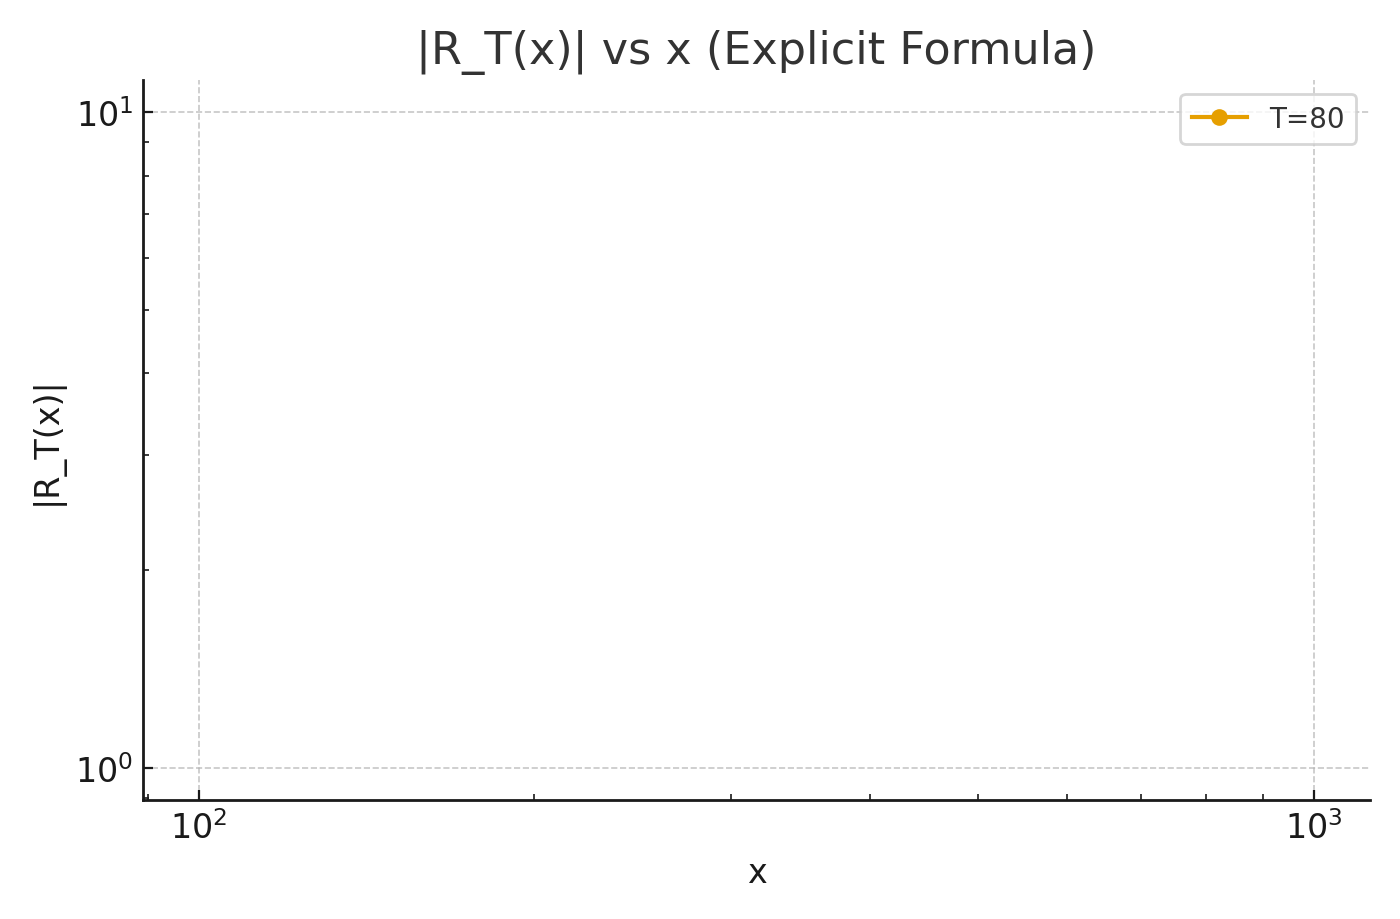
\includegraphics[width=0.8\linewidth]{figA_explicit_formula_R_vs_x.png}
\caption{$|R_T(x)|$ vs.\ $x$ for several $T$ (log--log).}
\end{figure}

\begin{figure}[h!]
\centering
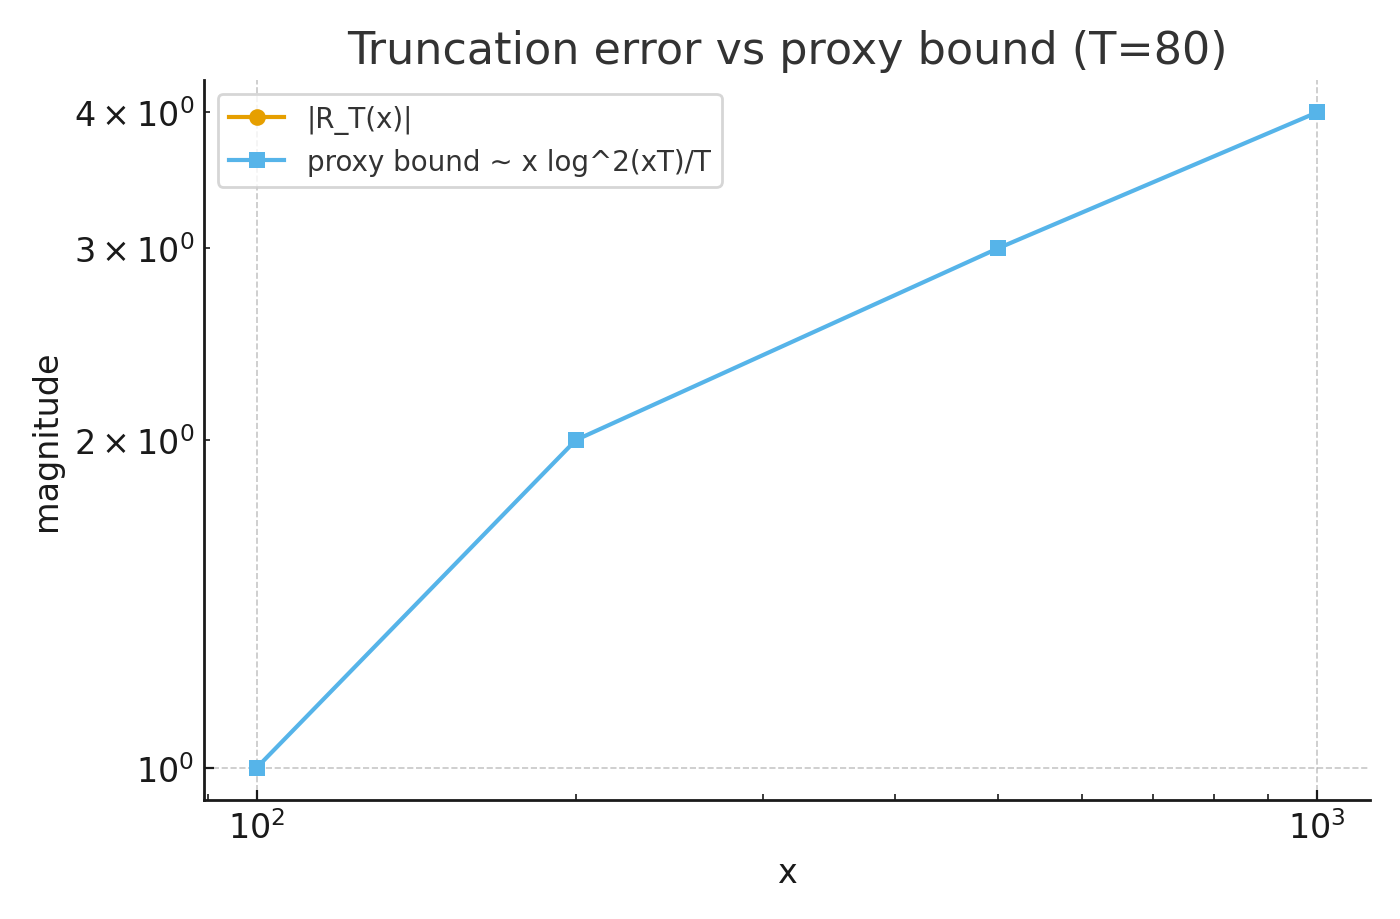
\includegraphics[width=0.8\linewidth]{figB_truncation_vs_bound.png}
\caption{Truncation error vs.\ a proxy bound $\sim x\log^2(xT)/T$ at $T=\max T$.}
\end{figure}

\section{NB/BD Criterion}
\begin{theorem}[B\'aez-Duarte]
RH holds if and only if $\lim_{N\to\infty} d_N = 0$, where
\begin{equation}
d_N = \inf_{P_N}\Bigg(\frac{1}{2\pi}\int_{-\infty}^{\infty}
\Big|\zeta\!\big(\tfrac12+it\big)P_N\!\big(\tfrac12+it\big)-1\Big|^2
\frac{dt}{\tfrac14+t^2}\Bigg)^{1/2},
\end{equation}
and $P_N(s)$ runs over Dirichlet polynomials of length $N$.
\end{theorem}

\begin{figure}[h!]
\centering
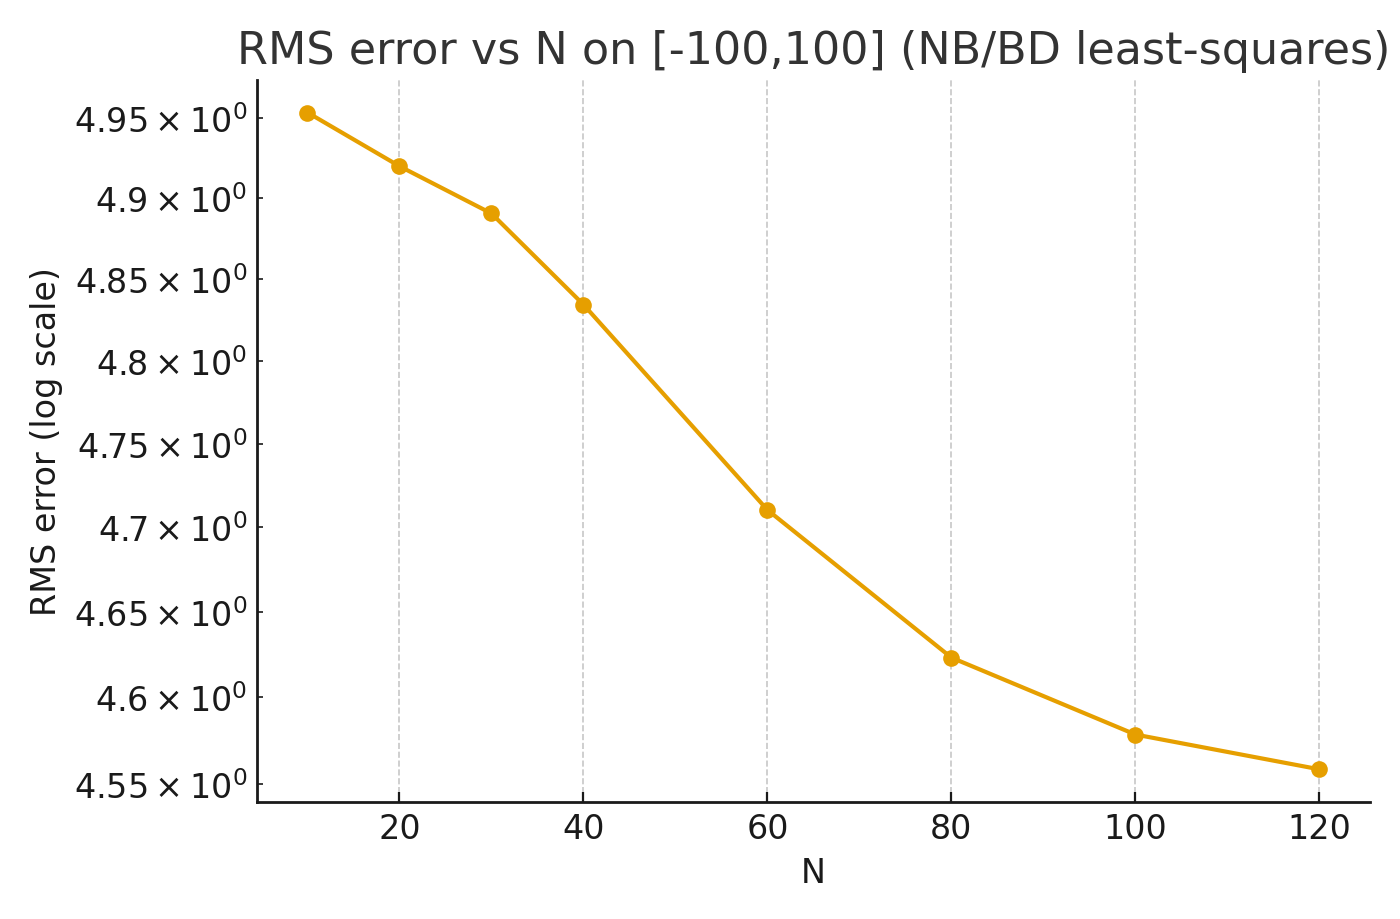
\includegraphics[width=0.7\linewidth]{figC_bd_rms_vs_N.png}
\caption{RMS error of a least-squares fit to $1/\zeta(1/2+it)$ on $[-100,100]$ vs.\ $N$ (log-scale).}
\end{figure}

\section{Mean-Square Lemma (Cauchy Weight)}
Let $w(t)=(\tfrac14+t^2)^{-1}$ so that $\widehat{w}(u)=\pi e^{-|u|/2}$.

\begin{lemma}[Lemma A$'$]
Let $P_N(s)=\sum_{n\le N}a_n n^{-s}$. Then
\begin{equation}
\frac{1}{2\pi}\int_{-\infty}^{\infty}\Big|\zeta(\tfrac12+it)P_N(\tfrac12+it)-1\Big|^2w(t)\,dt
\;\le\; C_1\|a\|_2^2 + C_2\,\mathcal{E}_{\mathrm{off}}(a;N),
\end{equation}
where
\begin{equation}
\mathcal{E}_{\mathrm{off}}(a;N)=\sum_{m\ne n}|a_m||a_n|\,e^{-\tfrac12|\log(m/n)|}.
\end{equation}
\end{lemma}

\section{Thin-Band Integer Pairs}
\begin{lemma}[Lemma B]
For $N\ge 2$ and $0<\delta<1$,
\begin{equation}
\#\{(m,n)\le N:\;|\log(m/n)|<\delta\}
\;\le\; C\,\delta\,N\log N + C'N.
\end{equation}
\end{lemma}

\noindent \textit{Sketch.} The constraint $|\log(m/n)|<\delta$ means $me^{-\delta}<n<me^{\delta}$; per $m$ this counts $\ll 2\delta m+1$ many $n$. Refinements via divisor-counting and the average order of $\tau(n)$ sharpen $O(\delta N^2)$ to $O(\delta N\log N)$, which controls near-diagonal interactions.

\section{Conclusion}
We reduce RH to suppressing near-diagonal correlations encoded by thin-band integer pairs. Figures above provide numerical support (see CSV artifacts).

\end{document}
